% =====================================================================
%  capitulos/cap15.tex — Capítulo 15. Lengua, dialecto y descripción
%  gramatical: el caso del español rioplatense
%  Autores: Carlos Muñoz Pérez y Andrés Saab
%  Fuente: Capitulo_15_normalizado.docx
% =====================================================================
\capitulo{Lengua, dialecto y descripción gramatical: el caso del español rioplatense}{Carlos Muñoz Pérez y Andrés Saab}

\section{Introducción}

Este capítulo ofrece una introducción al \termino{español rioplatense}, la
variedad del español hablada en la región del Río de la Plata (Argentina y
Uruguay). El recorrido comienza con una discusión sobre las nociones de
\textit{lengua} y \textit{dialecto}; como veremos, si bien ambos términos son de
uso habitual, es difícil distinguirlos desde un punto de vista estrictamente
gramatical. Luego, se presentan los factores históricos y geográficos que
moldearon la variedad rioplatense y se describen sus rasgos más distintivos en
los planos léxico, fonético-fonológico, morfológico y sintáctico. Entre los
fenómenos analizados y discutidos se incluyen el lunfardo, el yeísmo rehilado,
el voseo y el doblado de clíticos, entre otros.

\section{Algunas precisiones terminológicas sobre lengua y dialecto}\label{sec:15-terminologia}

El español rioplatense es una de las variedades del español habladas en América
del Sur. Antes de describir sus rasgos particulares, quisiéramos problematizar
dos términos que utilizamos a lo largo de este capítulo, \textit{lengua} y
\textit{dialecto}, ya que, aunque parecen nociones sencillas, veremos que son más
complejas de lo que suele suponerse.

\subsection{Lengua-I y lengua-E}\label{sec:15-lenguai}

El término \textit{lengua} puede significar al menos dos cosas distintas. En un
primer sentido, una lengua, como se planteó en el \capref{1}
(§\ref{sec:01-generativa}), es un tipo de conocimiento interno: algo que cada ser
humano desarrolla durante sus primeros años de vida gracias a la combinación de
(i) una capacidad biológica innata para el lenguaje y (ii) los estímulos
lingüísticos que recibe de su entorno. Este conocimiento es mental e individual:
está en la cabeza de cada hablante. En la tradición generativa, siguiendo una
distinción propuesta por \textcite{chomsky1986}, este objeto se denomina
\termino{lengua-I}. En un segundo sentido, \textit{lengua} puede referirse a un
objeto externo: el conjunto de expresiones y enunciados que una comunidad
produce y que pueden ser observados, recopilados y analizados. Cuando hablamos de
«el español» o «el guaraní» como entidades que existen más allá de cualquier
hablante individual, estamos usando esta segunda acepción. A este objeto lo
llamamos \termino{lengua-E}. Esta segunda acepción es, a grandes rasgos, la
concepción de lengua que ha predominado en la mayor parte de la tradición
lingüística, desde la gramática tradicional hasta el estructuralismo.

¿Cuál es la relación entre ambas nociones? Podemos pensarlo así: la lengua-I es
el mecanismo que cada hablante tiene en su mente y que le permite producir y
comprender oraciones; la lengua-E es el producto observable de ese mecanismo, es
decir, el conjunto de enunciados que efectivamente se producen. Ahora bien, esta
relación no es perfecta: en el uso de la lengua intervienen factores externos
(interrupciones y errores por cansancio, distracción, etc.) que introducen
«ruido» en los datos. Por eso, parte del trabajo del lingüista consiste en
determinar qué fragmentos de la lengua-E reflejan genuinamente la lengua-I de los
hablantes y cuáles son producto de esas interferencias.

Para entender mejor la distinción, pensemos en un caso concreto. Imaginemos a una
niña nacida en la provincia de Buenos Aires en la década de 1940. Su padre es un
inmigrante italiano que habla un dialecto del norte de Italia; su madre es una
inmigrante gallega que habla español y gallego. Ambos padres quieren que su hija
aprenda español, la lengua oficial del país, que será imprescindible para su
escolarización. Además, tenemos que considerar que las lenguas de los inmigrantes
están fuertemente estigmatizadas. Por tanto, ¿qué datos lingüísticos recibe esta
niña? Podemos suponer que se trata de un conjunto bastante caótico: fragmentos de
español peninsular y de gallego (de su madre), fragmentos de un dialecto de
Italia (de su padre) y español rioplatense (de vecinos, familiares y, más tarde,
de la escuela). Esos estímulos lingüísticos no provienen de una única lengua-I,
ni constituyen un conjunto homogéneo, sino que son ejemplos de distintas
lenguas-E. Y, sin embargo, en un plazo relativamente breve, la niña comienza a
producir oraciones que responden a un sistema gramatical completo: su propia
lengua-I. Esta historia se repitió en innumerables hogares de Buenos Aires
durante las grandes olas migratorias: cada niño o niña desarrolló una lengua-I
estrictamente individual, pero, como los factores externos eran en gran medida
similares, sus producciones lingüísticas comparten numerosas propiedades
fonéticas, fonológicas, morfológicas y sintácticas. Ese conjunto de propiedades
compartidas es, justamente, lo que describimos cuando hablamos del español
rioplatense.

\begin{destacado}
\textbf{Para tener en cuenta.} Idealmente, una descripción completa de una lengua
o de un dialecto debería capturar ese conocimiento interno que cada persona
adquiere, es decir, debería ser una teoría acerca de la lengua-I. No obstante,
dada la naturaleza introductoria de este capítulo, lo que ofrecemos es una
recopilación de ciertos fragmentos de lengua-E. Para decirlo de otro modo,
presentamos un subconjunto de los datos lingüísticos que caracterizan de manera
diferencial al español hablado hoy en día en el área rioplatense.
\end{destacado}

\subsection{La escurridiza noción de dialecto}\label{sec:15-dialecto}

Pasemos entonces a una pregunta central: ¿existe alguna relación relevante entre
las nociones de \textit{lengua} y \textit{dialecto}? Lo primero que debemos hacer
es descartar una idea muy extendida, pero incorrecta: que un dialecto es una
«desviación» o una versión «inferior» de una lengua. En el uso popular, el
concepto de \textit{dialecto} suele referirse a formas no estándares de hablar, a
veces consideradas rústicas o inferiores, o a lenguas minoritarias sin estatus
oficial. Así, por ejemplo, en México es habitual oír que las comunidades
indígenas hablan «dialectos», en contraste con el español, que sí sería una
«lengua». Así presentada, esta distinción no tiene sustento lingüístico y la
rechazamos explícitamente.

Un criterio algo más sofisticado, pero igualmente problemático, es el de la
\termino{intercomprensión}: según este criterio, dos variedades son dialectos de
una misma lengua si sus hablantes pueden entenderse entre sí y, en cambio, son
lenguas distintas si no pueden hacerlo. El problema es que este criterio no
funciona de manera consistente. Hay lenguas reconocidas como tales que son mucho
más parecidas entre sí que ciertos dialectos de una misma lengua. El español y el
portugués, por ejemplo, son lenguas oficiales de estados distintos y se
consideran lenguas diferentes, pero un hablante del español rioplatense y un
hablante del portugués brasileño pueden entenderse con relativa facilidad en
muchas situaciones cotidianas. A su vez, hay diferencias específicas entre, por
ejemplo, el español caribeño hablado en República Dominicana y el español
rioplatense que pueden dificultar la mutua intercomprensión. Este criterio, por
tanto, no nos ofrece una frontera clara y sistemática.

¿Cómo definir entonces \textit{dialecto} de manera rigurosa?
\textcite{silvacorvalan2001} propone una solución práctica: si tomamos una
lengua-E como el español y la delimitamos a partir de factores históricos,
políticos, geográficos y culturales, podemos pensar que se organiza internamente
como una pirámide. En la cúspide de esta \termino{pirámide dialectal} se ubica la
lengua histórica o común (es decir, «el español» a nivel general); en un nivel
intermedio, los grandes dialectos regionales (es decir, el español peninsular y
el español de América); y en la base, los dialectos locales concretos (aquí es
donde encontramos el rioplatense, el español andaluz, etc.). Un punto importante
de esta concepción es que supone que la lengua general no es hablada por ninguna
comunidad en particular: lo que cada persona habla es siempre un dialecto
particular, situado en la base de la pirámide. En otras palabras, hablar una
lengua equivale siempre a hablar un dialecto de esa lengua. La
figura~\ref{fig:15-piramide} ilustra esta organización.

\begin{figure}[htbp]
  \centering
  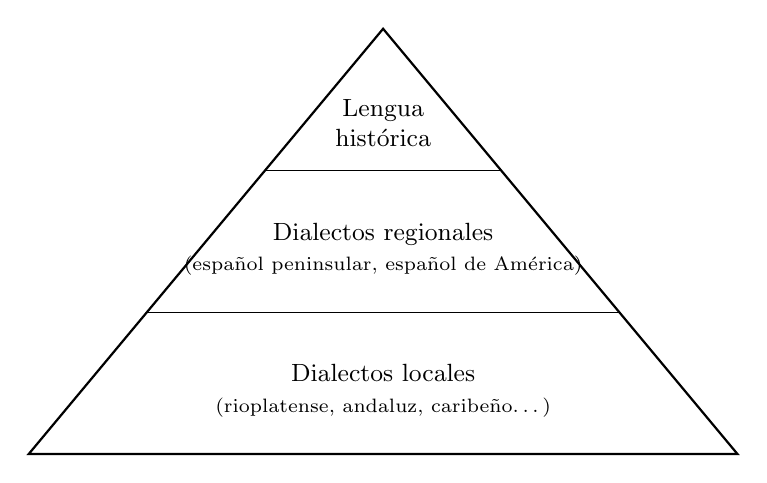
\begin{tikzpicture}[x=1mm,y=1mm,font=\small]
    \draw[thick] (0,0) -- (90,0) -- (45,54) -- cycle;
    \draw (15,18) -- (75,18);
    \draw (30,36) -- (60,36);
    \node[align=center] at (45,42) {Lengua\\histórica};
    \node[align=center] at (45,26) {Dialectos regionales\\\scriptsize(español peninsular, español de América)};
    \node[align=center] at (45,8) {Dialectos locales\\\scriptsize(rioplatense, andaluz, caribeño\ldots)};
  \end{tikzpicture}
  \caption{Pirámide dialectal \parencite[adaptado de][14]{silvacorvalan2001}}\label{fig:15-piramide}
\end{figure}

\pendiente{Diagrama 1 sin imagen en el original; reconstruido a partir del texto}

Ahora bien, en un esquema como el de Silva-Corvalán, lo que ocupa la cúspide de
la pirámide, es decir, la «lengua histórica o común», no se define por criterios
puramente lingüísticos. Como ya se observó, son factores históricos,
geográficos, culturales y, de manera decisiva, políticos los que determinan qué
cuenta como «lengua» y qué cuenta como «dialecto». Es decir, lo que nos lleva a
clasificar el español rioplatense, el español caribeño o el español andaluz como
«dialectos del español» y no como lenguas independientes no es un criterio
gramatical, sino el hecho de que comparten una tradición histórica, geográfica y
cultural, un nombre y, sobre todo, un marco político-institucional que los
agrupa bajo una misma etiqueta.

\begin{ejercicio}\label{ej:15-weinreich}
Al lingüista Max Weinreich se le atribuye el aforismo «una lengua es un dialecto
con un ejército y una marina». Discuta el sentido de esta afirmación a la luz de
la discusión precedente. Específicamente: ¿a qué tipo de criterio para
distinguir \textit{lengua} de \textit{dialecto} refiere el aforismo?
\end{ejercicio}

\subsection{Una posible diferenciación: microparámetros frente a macroparámetros}\label{sec:15-parametros}

Cabe preguntarse, entonces, si existe alguna manera «lingüística» de establecer
una distinción entre lenguas y dialectos. Como veremos, la respuesta es «sí»,
pero bajo ciertos supuestos. Primero, debemos suponer que existen distintas
maneras en las que las lenguas pueden diferir entre sí. La idea es que existen
«opciones de configuración» del sistema lingüístico denominadas
\termino{parámetros} (véase el \capref{1}, §\ref{sec:01-generativa}), que se
fijan durante el proceso de adquisición de la lengua. Algunas de las propiedades
que determinan estos parámetros afectan a todo el sistema de la lengua y crean
una especie de «efecto dominó» con respecto al funcionamiento de varias áreas de
la gramática. Estos parámetros «de gran alcance» se denominan por lo general
\termino{macroparámetros}.\footnote{\textcite{roberts2019} propone una tipología
más fina, que distingue al menos cuatro niveles de variación paramétrica (macro-,
meso-, micro- y nanoparámetros), ordenados según el grado de especificidad del
cambio observado. Por simplicidad, en este capítulo trabajamos solo con el
contraste entre macro- y microparámetros.} Por ejemplo, muchas veces se asume
que existe un macroparámetro encargado del orden de las palabras dentro de los
sintagmas: en lenguas como el español, el núcleo aparece al inicio del sintagma;
en lenguas como el japonés, el núcleo aparece al final.

\begin{exe}
  \ex\label{ex:15-espanol} Núcleo inicial (español):
    \begin{xlist}
      \ex {}[\etq{SV} comprar un regalo]
      \ex {}[\etq{SP} en la ciudad]
    \end{xlist}
  \ex\label{ex:15-japones} Núcleo final (japonés):
    \begin{xlist}
      \ex
        \gll {}[\etq{SV} purezento-o kau]\\
             {} regalo-\textsc{acus} comprar\\
        \glt \sig{comprar un regalo}
      \ex
        \gll {}[\etq{SP} machi-de]\\
             {} ciudad-en\\
        \glt \sig{en la ciudad}
    \end{xlist}
\end{exe}

Por otra parte, la bibliografía también ha identificado parámetros de variación
que describen diferencias más «pequeñas» o de alcance más restringido. Estos se
conocen con el nombre de \termino{microparámetros}. Los microparámetros describen
cambios en las propiedades de los elementos funcionales de la lengua (p.~ej., en
pronombres, en morfemas flexivos, en artículos), básicamente en unidades de
clase cerrada dentro del sistema lingüístico. Así, por ejemplo, podemos concebir
el llamado \termino{leísmo} como un caso de variación microparamétrica en el
sistema de pronombres clíticos de ciertos dialectos del español. El leísmo
consiste en el uso del pronombre \forma{le} (originalmente dativo) en contextos
en los que otros dialectos emplean los pronombres acusativos \forma{la} o
\forma{lo}. Así, para referirse a una misma situación (por ejemplo, haber visto a
una persona el día anterior), un hablante de un dialecto no leísta y uno de un
dialecto leísta producirían oraciones distintas.

\begin{exe}
  \ex\label{ex:15-leismo}
    \begin{xlist}
      \ex La hemos visto ayer. \hfill \textit{variante no leísta}
      \ex Le hemos visto ayer. \hfill \textit{variante leísta}
    \end{xlist}
\end{exe}

A partir de la distinción entre macroparámetros y microparámetros es posible
ofrecer una definición explícita de lo que es una lengua y de lo que es un
dialecto. Así, si dos sistemas lingüísticos (es decir, dos lenguas-I en un
sentido técnico) difieren en su configuración macroparamétrica, podría decirse
que son lenguas diferentes (p.~ej., el español y el japonés son lenguas
diferentes porque, como muestran los ejemplos de \exref{ex:15-espanol} y
\exref{ex:15-japones}, difieren en al menos un macroparámetro). En cambio, si dos
sistemas lingüísticos solo difieren en términos de sus microparámetros, porque
sus macroparámetros están configurados de manera análoga, puede decirse que son
dialectos de la misma lengua (p.~ej., las variantes leístas y no leístas de
\exref{ex:15-leismo} representarían dialectos de la misma
lengua).\footnote{Esta es, en esencia, la propuesta de \textcite{baker2008}.}

Esta manera de entender qué es una lengua y qué es un dialecto descansa sobre la
distinción entre macroparámetro y microparámetro. Sin embargo, no todos los
lingüistas acuerdan en que ambas nociones son necesarias. Algunos autores
defienden la idea de que los macroparámetros no existen como tales y que las
grandes diferencias que se observan a nivel interlingüístico se deben
simplemente a la acumulación de diferencias microparamétricas. La idea suele
sintetizarse en la siguiente tesis de \textcite{kayne2005}:

\begin{exe}
  \ex\label{ex:15-kayne} Todo parámetro es un microparámetro.
\end{exe}

Bajo este supuesto, no existen distintos tipos de parámetro que justifiquen una
distinción cualitativa entre lengua y dialecto; es decir, dado que toda unidad
de cambio lingüístico es de la misma naturaleza, los términos \textit{lengua} y
\textit{dialecto} refieren al mismo tipo de variación. La única diferencia que
puede establecerse entre ambas nociones es, a lo sumo, de grado: el español y el
japonés serían lenguas distintas porque acumulan entre sí muchas pequeñas
diferencias; el español rioplatense y el español caribeño serían dialectos del
español porque acumulan entre sí muchas menos diferencias.

A pesar de nublar la distinción entre lengua y dialecto, esta segunda postura
tiene una consecuencia práctica interesante: convierte a la dialectología en una
herramienta de investigación poderosa para la teoría lingüística. Si la
variación entre dialectos es del mismo tipo que la variación entre lenguas,
entonces comparar dialectos cercanos nos permite aislar diferencias mínimas y
estudiar sus efectos en detalle, como en una suerte de experimento controlado.

\section{Cuestiones históricas y geográficas}\label{sec:15-historia}

Para contextualizar las propiedades del español rioplatense, es necesario conocer
algunos hechos históricos que incidieron directamente en la conformación de esta
variedad. No se trata de hacer un recorrido exhaustivo por la historia de la
región, sino de identificar los momentos clave en los que ciertos eventos
demográficos y políticos dejaron una huella en la lengua.

La fundación definitiva de Buenos Aires tuvo lugar en 1580, con la expedición de
Juan de Garay. De los sesenta y seis participantes de esa expedición, solo diez
provenían directamente de España; el resto eran mestizos procedentes de Asunción
\parencite{fontanella1987}. Esto significa que, desde sus orígenes, Buenos Aires
fue una ciudad donde convivían el español y el guaraní: una parte considerable de
sus primeros pobladores, en particular las mujeres, eran hablantes bilingües de
ambas lenguas. Esta situación inicial de contacto lingüístico se fue modificando
a lo largo de los siglos \textsc{xvii} y \textsc{xviii}, a medida que la llegada
de nuevos pobladores desde España impuso progresivamente el uso del español por
sobre el guaraní. Hacia 1776, con el establecimiento definitivo del Virreinato
del Río de la Plata, Buenos Aires se consolidó como centro administrativo y
cultural de la región, lo que reforzó el papel institucional del español como
lengua dominante.

Sin embargo, el factor histórico que más profundamente moldeó el perfil
lingüístico del español rioplatense fue la inmigración masiva de fines del siglo
\textsc{xix} y principios del \textsc{xx}. Como destaca
\textcite{ditullio2010a}, las políticas inmigratorias del Estado argentino,
consolidado hacia 1880, transformaron de manera drástica el panorama cultural y
lingüístico de la región. Para dimensionar la magnitud de este cambio, basta
considerar algunos datos: entre 1869 y 1914, la población del país se
cuadruplicó, pasando de aproximadamente dos millones a casi ocho millones de
habitantes. Hacia la época del Centenario (1910), uno de cada tres habitantes era
extranjero. De los cuatro millones de inmigrantes registrados en 1914, la mitad
eran italianos provenientes tanto del norte como del sur de Italia. Estos
hablantes, que traían consigo una enorme diversidad de dialectos italianos,
ejercieron una influencia considerable sobre el español de la zona,
especialmente en el plano de la entonación, la morfología y el
léxico.\footnote{Debe tenerse en cuenta, sin embargo, que, según
\textcite[94]{fontanella1987}, varias propiedades fonológicas y fonéticas de la
variedad, como el seseo, el yeísmo y la aspiración y elisión de /s/, ya habían
comenzado a consolidarse en el siglo \textsc{xviii}, antes de las grandes olas
migratorias (véase §\ref{sec:15-fonetica}).}

\subsection{El español rioplatense}\label{sec:15-rioplatense}

Ahora bien, es importante no confundir el español rioplatense con el español
argentino en general. La Argentina es un país extenso y, desde el punto de vista
dialectológico, presenta una diversidad interna que a menudo pasa inadvertida. En
un trabajo clásico, \textcite{vidal1964} distingue al menos cinco regiones
dialectales dentro del territorio argentino, muchas de las cuales se extienden
más allá de las fronteras nacionales.

\begin{exe}
  \ex\label{ex:15-regiones} Regiones dialectales de la Argentina
      \parencite{vidal1964}:
    \begin{xlist}
      \ex La \textit{región rioplatense}, que es el objeto de estudio de este
          capítulo.
      \ex La \textit{región guaranítica}, que comprende Corrientes, Misiones, el
          este de Formosa y del Chaco, el extremo noreste de Santa Fe y, de manera
          menos clara, zonas de Entre Ríos.
      \ex La \textit{región del noroeste}, que abarca Jujuy, Salta, Tucumán,
          Santiago del Estero, Catamarca, La Rioja, el norte de San Juan y San Luis
          y el noroeste de Córdoba.
      \ex La \textit{región de Cuyo}, que incluye Mendoza, San Juan y el norte de
          Neuquén.
      \ex La \textit{región central}, constituida principalmente por Córdoba y San
          Luis.
    \end{xlist}
\end{exe}

\figurapendiente{Regiones dialectales de la Argentina (adaptado de Vidal de Battini, 1964). Fuente: Wikimedia Commons, licencia CC BY-SA 3.0}{fig:15-mapa}

\begin{destacado}
\textbf{Para tener en cuenta.} La clasificación anterior permite apreciar que lo
que solemos llamar «español argentino» es en realidad un mosaico de variedades
con rasgos propios. Un hablante de Salta y un hablante de Buenos Aires comparten
la nacionalidad, pero sus maneras de hablar presentan diferencias notables en la
pronunciación, el vocabulario y ciertas construcciones gramaticales. El español
rioplatense es solo una de esas variedades y no debe tomarse como representativa
de todo el país.
\end{destacado}

¿Qué territorio abarca, entonces, el español rioplatense? Según
\textcite{vidal1964}, esta región incluye la provincia de Buenos Aires, la ciudad
de Buenos Aires, las provincias de Santa Fe, Entre Ríos y La Pampa, las zonas de
la Patagonia colonizadas por población proveniente de Buenos Aires y,
finalmente, amplias zonas del Uruguay. Se trata, en palabras de la autora, de
«la región lingüística más extensa y más europeizada de la República»
\parencite[76]{vidal1964}.

Un último punto merece atención. Como señalan \textcite[12]{ditullio2011}, el
español rioplatense no se corresponde con ninguna unidad política: no coincide
con las fronteras de un estado-nación, sino que se extiende a ambos lados del Río
de la Plata, abarcando territorio argentino y uruguayo. Esta observación, que
puede parecer obvia, tiene implicaciones importantes: nos recuerda que las
fronteras lingüísticas y las fronteras políticas rara vez coinciden. A pesar de
los intentos de homogeneización lingüística llevados adelante por el Estado
argentino entre fines del siglo \textsc{xix} y la primera mitad del \textsc{xx},
la diversidad dialectal del país sigue siendo rica y, en buena medida,
insuficientemente estudiada.

Veamos, entonces, cuáles son las particularidades que caracterizan al español de
la zona del Río de la Plata.

\section{Léxico}\label{sec:15-lexico}

Las lenguas no solo se diferencian por su pronunciación o su gramática: el
vocabulario es muchas veces el rasgo que los hablantes perciben con mayor
facilidad. En el caso del español rioplatense, el léxico presenta
particularidades que reflejan de manera directa la historia de contacto
lingüístico que describimos en la sección anterior.

En términos generales, las variedades del español del Cono Sur comparten un
conjunto de palabras tomadas de lenguas indígenas americanas, en particular del
quechua.

\begin{exe}
  \ex\label{ex:15-quechua} Préstamos del quechua en el español rioplatense:
    \begin{xlist}
      \ex \forma{cancha} (\sig{terreno delimitado para practicar deportes o
          realizar actividades})
      \ex \forma{choclo} (\sig{maíz tierno})
      \ex \forma{papa} (\sig{tubérculo comestible})
      \ex \forma{poroto} (\sig{tipo de legumbre})
    \end{xlist}
\end{exe}

En menor medida, el español rioplatense también conserva algunas voces de origen
guaraní, testimonio del contacto temprano entre ambas lenguas en la región del
Río de la Plata, según se señaló en §\ref{sec:15-historia}.

\begin{exe}
  \ex\label{ex:15-guarani} Préstamos del guaraní en el español rioplatense:
    \begin{xlist}
      \ex \forma{gurí} (\sig{niño})
      \ex \forma{pororó} (\sig{pochoclo} o \sig{palomitas de maíz})
      \ex \forma{yacaré} (\sig{tipo de caimán})
      \ex \forma{ananá} (\sig{piña})
    \end{xlist}
\end{exe}

Estas voces son de uso cotidiano en el español rioplatense, y muchos hablantes
las emplean sin saber que provienen de lenguas indígenas. La distribución de
estos préstamos no es homogénea entre las distintas variedades del español
americano: muchas voces de origen indígena que son comunes en una región resultan
desconocidas en otra. Estas diferencias se explican, en parte, por la diversidad
de \termino{lenguas de sustrato}\footnote{Se denominan \textit{lenguas de
sustrato} las lenguas que, en una situación de contacto lingüístico, son habladas
por la población originaria de un territorio cuando se impone una lengua
dominante (la lengua de superestrato). Aunque eventualmente la lengua de sustrato
puede dejar de hablarse, suele dejar huellas en la lengua dominante (típicamente
en el léxico, pero también en la fonética y la sintaxis). En el caso del español
americano, las lenguas indígenas de cada región funcionaron generalmente como
sustrato.} que han intervenido en la conformación léxica de cada variedad.

Sin embargo, el rasgo más distintivo del léxico rioplatense no son los
indigenismos, sino el llamado \termino{lunfardo}. ¿Qué es el lunfardo? En términos
simples, se trata de un conjunto de palabras y expresiones coloquiales,
originalmente asociadas al habla popular de Buenos Aires, que se han ido
incorporando al uso cotidiano de los hablantes rioplatenses a lo largo de más de
un siglo. Quien dice \forma{laburo} en lugar de \forma{trabajo}, \forma{mango} en
lugar de \forma{peso} (la moneda) o \forma{afanar} en lugar de \forma{robar}
está usando lunfardo, muchas veces sin ser consciente de ello. El lunfardo es un
repertorio dinámico y en constante transformación: cada generación incorpora
nuevas voces y deja de usar otras.\footnote{Varios de los fenómenos gramaticales
discutidos en este capítulo han sido estigmatizados por estar asociados al
lunfardo, que muchos veían como una jerga delictiva. Véanse
\textcite{gobello2001} y \textcite{conde2009} para una postura que reivindica el
lunfardo como una manifestación cultural legítima y un componente esencial de la
identidad rioplatense.}

La riqueza del lunfardo es el resultado de una interacción compleja entre varios
factores: la literatura y la música argentinas de comienzos del siglo
\textsc{xx} (en particular el tango, que difundió muchas de estas voces), el
proceso de consolidación de la variedad rioplatense y, de manera fundamental, la
contribución de los inmigrantes italianos y de sus dialectos.

\begin{recuadro}[¿Qué es el lunfardo?]
Según \textcite[14]{conde2004}, el lunfardo se conformó en su origen con términos
traídos por la inmigración, pero no es un vocabulario cerrado: hay un único
lunfardo, que en las décadas sucesivas se amplió con palabras provenientes de
ámbitos muy diversos, casi todas de creación local y sobre la base de la lengua
española. El lenguaje del fútbol y el del turf, las jergas de oficios y
profesiones, los ambientes de la droga, el mundo del rock y de las «tribus
urbanas», la jerga del psicoanálisis, la radio y la televisión, entre otros, han
aportado una cantidad innumerable de vocablos, extendidos ya a todo el espectro
social de buena parte del país.\pendiente{El original transcribe una cita
textual de Conde (2004, p.~14) de unas 120 palabras; se parafraseó: decidir si
se restituye}
\end{recuadro}

Numerosos términos del lunfardo son de origen italiano.

\begin{exe}
  \ex\label{ex:15-italianismos} Italianismos en el lunfardo rioplatense:
    \begin{xlist}
      \ex \forma{laburo} (\sig{trabajo}, del italiano \forma{lavoro})
      \ex \forma{birra} (\sig{cerveza}, del italiano \forma{birra})
      \ex \forma{bochar} (\sig{reprobar un examen}, del italiano
          \forma{bocciare})
      \ex \forma{gamba} (\sig{pierna}, del italiano \forma{gamba})
      \ex \forma{nona} (\sig{abuela}, del italiano \forma{nonna})
      \ex \forma{napia} (\sig{nariz}, del genovés \forma{nàppia}, \sig{nariz
          grande})
    \end{xlist}
\end{exe}

En menor medida, el lunfardo también incorporó voces de otras lenguas y
registros, como el francés, el portugués, el caló peninsular (la lengua de los
gitanos españoles), el guaraní y el quechua \parencite{conde2009}.

Un mecanismo particularmente interesante de creación léxica dentro del lunfardo
es el llamado \termino{vesre}. El término mismo ya nos da una pista de en qué
consiste: \forma{vesre} es la inversión silábica de la palabra \forma{revés}. El
procedimiento toma una palabra del léxico rioplatense y reordena sus sílabas, lo
que produce una forma con el mismo significado referencial, pero con un valor
expresivo diferente, generalmente más coloquial o lúdico.\footnote{Véase
\textcite{bohrn2015} para un análisis detallado de este fenómeno.}

\begin{exe}
  \ex\label{ex:15-vesre} Ejemplos de vesre en el español rioplatense:
    \begin{xlist}
      \ex \forma{café} $\rightarrow$ \forma{feca}
      \ex \forma{mujer} $\rightarrow$ \forma{jermu}
      \ex \forma{tango} $\rightarrow$ \forma{gotán}
      \ex \forma{pagar} $\rightarrow$ \forma{garpar}
    \end{xlist}
\end{exe}

Algunas formas de vesre se han convencionalizado de tal manera que su origen
resulta opaco, incluso para los propios hablantes rioplatenses. Un ejemplo
clásico es \forma{ortiba}, que significa \sig{delator} o \sig{aguafiestas}: pocos
hablantes reconocen que se trata de la inversión de \forma{batidor}, una palabra
del lunfardo que significa \sig{el que delata}.

El léxico del español rioplatense constituye, entonces, un terreno donde se
pueden rastrear con claridad las huellas del contacto lingüístico y de la
historia social de la región. En las secciones siguientes veremos que la
pronunciación, la morfología y la sintaxis de esta variedad presentan, cada una a
su manera, el mismo tipo de singularidad.

\begin{ejercicio}\label{ej:15-prestamos}
En la sección sobre léxico se presentaron préstamos del quechua, del guaraní y
del italiano en el español rioplatense. Elija tres palabras de uso cotidiano en
su variedad del español que sospeche que provienen de una lengua indígena o de
una lengua de inmigración. Investigue su etimología y discuta: ¿los hablantes son
generalmente conscientes del origen de estas palabras?
\end{ejercicio}

\section{Fonética y fonología}\label{sec:15-fonetica}

En esta sección describimos las propiedades más salientes de la pronunciación
del español rioplatense. Para representar los sonidos del habla, utilizamos el
Alfabeto Fonético Internacional (AFI), que se introdujo en el \capref{3}
(§\ref{sec:03-transcripcion}), un sistema de notación estándar en lingüística que
permite distinguir con precisión entre la forma escrita de una palabra y su
pronunciación efectiva. Como se vio en ese capítulo, las transcripciones
fonéticas aparecen entre corchetes ([~]), mientras que las representaciones
fonológicas aparecen entre barras (/~/).

Comenzamos por las propiedades \textit{segmentales}, es decir, las que conciernen
a los sonidos individuales (consonantes y vocales), para luego pasar a las
propiedades \textit{prosódicas}, que tienen que ver con la melodía y el ritmo del
habla. Recordemos que, como se dijo en el \capref{3}, al igual que la mayoría de
las variedades americanas del español, el rioplatense presenta \termino{seseo}:
la ausencia de la fricativa dental sorda /θ/, que en algunas variedades
peninsulares permite distinguir los grafemas <c> / <z> de la letra <s>. En
consecuencia, pares como \forma{casa} y \forma{caza} se pronuncian de manera
idéntica:

\begin{exe}
  \ex\label{ex:15-seseo} Seseo: \forma{casa}, \forma{caza} $\rightarrow$
      \fon{ˈka.sa}
\end{exe}

Este rasgo no es exclusivo del rioplatense, sino que lo comparte con
prácticamente todo el español americano. Más allá del seseo, el español
rioplatense presenta cuatro rasgos segmentales más o menos distintivos que
describimos a continuación.

En primer lugar, el rioplatense tiende a aspirar la /s/ cuando esta se encuentra
al final de una sílaba y antes de otra consonante.

\begin{exe}
  \ex\label{ex:15-aspiracion} Aspiración de /s/ en coda
      preconsonántica:\footnote{El concepto de coda silábica se introdujo en el
      \capref{3}, §\ref{sec:03-silaba}.}
    \begin{xlist}
      \ex \forma{asco} $\rightarrow$ \fon{ˈah.ko}
      \ex \forma{es lo mismo} $\rightarrow$ \fon{ˈeh.lo.ˈmih.mo}
    \end{xlist}
\end{exe}

\pendiente{El original transcribe \fon{ˈah.co}; se corrigió a \fon{ˈah.ko}}

También se observa la elisión completa de la /s/, especialmente al final de
palabra, aunque la aspiración es el fenómeno más frecuente. Este rasgo es
compartido con otras variedades del español argentino
\parencite{terrell1978,donni1984}.

En segundo lugar, el rioplatense exhibe patrones de diptongación de vocales
medias \parencite{luis1983}. En ciertos contextos, las vocales /e/ y /o/, cuando
están en contacto con otra vocal, tienden a pronunciarse como diptongos.

\begin{exe}
  \ex\label{ex:15-diptongacion} Diptongación de vocales medias:
    \begin{xlist}
      \ex \forma{línea} $\rightarrow$ \fon{ˈli.nja}
      \ex \forma{almohada} $\rightarrow$ \fon{al.ˈmwa.da}
    \end{xlist}
\end{exe}

En tercer lugar, se observa una pérdida progresiva de la distinción entre /ɲ/ y
la secuencia /nj/. La <ñ> del español (técnicamente, una consonante nasal que se
articula con la lengua contra el paladar) tiende a confundirse con la secuencia
formada por <n> + <i> seguida de vocal
\parencite{colantoni2013hualde,bongiovanni2015}. En la práctica, esto significa
que las secuencias ortográficas <ña>, <ñe>, <ño>, <ñu> no siempre se distinguen
de <nia>, <nie>, <nio>, <niu> en la pronunciación.

\begin{exe}
  \ex\label{ex:15-nj} Pérdida de la distinción /ɲ/ frente a /nj/:
      \forma{huraño}, \forma{uranio} $\rightarrow$ \fon{u.ˈɾa.njo}
\end{exe}

Por último, quizá el rasgo más emblemático del español rioplatense sea su forma
particular de \termino{yeísmo}, que se conoce como \termino{yeísmo rehilado}. El
término \textit{rehilamiento} alude a la fricción intensa o vibración acústica
característica de este tipo de sonidos sibilantes. En la mayoría de las
variedades yeístas del español, los grafemas <ll> e <y> se pronuncian de manera
idéntica, con una fricativa palatal sonora \fon{ʝ}. En el rioplatense, en cambio,
ambos grafemas se realizan mediante una consonante fricativa que se produce con
la lengua en una posición más adelantada, similar a la de <sh> en inglés
\parencite[entre muchos otros]{zamora1949,guitarte1955}. Además, se observa una
tendencia histórica al ensordecimiento de este sonido: mientras que las
generaciones mayores suelen producir una variante sonora \fon{ʒ} (similar a la
<j> del francés \forma{je}), los hablantes más jóvenes tienden a usar una
variante sorda \fon{ʃ} (similar a la <sh> del inglés \forma{she}).\footnote{Se
puede consultar \textcite{rohena2013} para una discusión detallada del proceso de
ensordecimiento.}

\begin{exe}
  \ex\label{ex:15-rehilado} Yeísmo rehilado:
    \begin{xlist}
      \ex \forma{pollo} $\rightarrow$ \fon{ˈpo.ʒo} (variante sonora,
          generalmente asociada a hablantes mayores)
      \ex \forma{pollo} $\rightarrow$ \fon{ˈpo.ʃo} (variante sorda,
          generalmente asociada a hablantes jóvenes)
    \end{xlist}
\end{exe}

Además de sus sonidos particulares, el español rioplatense se distingue por su
\termino{entonación}: la «melodía» con la que los hablantes producen las
oraciones. Se trata de un rasgo que los propios hablantes de otras variedades del
español perciben con facilidad y que, como veremos, tiene una conexión histórica
con la inmigración italiana.

Un primer rasgo prosódico distintivo es la llamada \termino{alineación temprana
del pico tonal}, que afecta a los acentos prenucleares, es decir, a los acentos
que preceden al acento más prominente del enunciado. En la mayoría de las
variedades del español, cuando un hablante pronuncia una oración declarativa
neutra, el punto más alto de la curva melódica ---el pico tonal--- tiende a
ubicarse después de la sílaba acentuada, en la sílaba siguiente. En el español
rioplatense, en cambio, ese pico se produce tempranamente dentro de la sílaba
acentuada, un patrón que se asemeja a lo que se observa en varias lenguas
habladas en Italia \parencite{colantoni2004}; la figura~\ref{fig:15-pico}
esquematiza este contraste.

\figurapendiente{Patrones de alineación del pico tonal en acentos de oraciones declarativas neutras (adaptado de Colantoni y Gurlekian, 2004)}{fig:15-pico}

El acento nuclear, es decir, el último y más prominente del enunciado, presenta
un comportamiento distinto, aunque igualmente característico. En el rioplatense,
la melodía desciende de manera abrupta dentro de la propia sílaba acentuada y
alcanza el punto más bajo de todo el enunciado en un lapso muy breve, en lo que
\textcite{kaisse2001} denomina una «larga caída». En otras variedades del
español, esta caída final es más gradual y se distribuye a lo largo de más
sílabas. El resultado auditivo en el rioplatense es una melodía que parece
«cortarse» abruptamente al final de la oración. Este patrón es también
característico de las lenguas de Italia habladas por una parte significativa de
los inmigrantes que se asentaron en Buenos Aires.

\textcite{colantoni2004} interpretan estos patrones como el resultado de un
proceso de convergencia: dos sistemas entonativos, el español y el italiano, que
ya eran tipológicamente similares, se volvieron aún más parecidos a consecuencia
del contacto. La influencia del italiano sobre el español rioplatense habría sido
tanto directa (contacto cotidiano con hablantes italianos) como indirecta, a
través del lunfardo y del \termino{cocoliche}.\footnote{\textit{Cocoliche} es el
nombre que recibe el español hablado por los inmigrantes, principalmente
italianos, llegados a Buenos Aires entre las últimas décadas del siglo
\textsc{xix} y las primeras del \textsc{xx}. Se trata del resultado de la
adquisición incompleta del español por parte de hablantes adultos, con fuerte
interferencia de su lengua de origen.}

Otro rasgo prosódico relevante es la posibilidad de acentuar los pronombres
clíticos cuando estos aparecen después del verbo. Estos son pronombres como
\forma{lo, la, me, se}, que normalmente no llevan acento propio y que se apoyan
prosódicamente en el verbo (véase el \capref{10}, §\ref{sec:10-tonicos}). En el
común de las variedades del español, cuando un clítico se añade al final de un
verbo (por ejemplo, \forma{aGÁrrenlo, DÁmelo}), el acento permanece en la sílaba
acentuada del verbo. En el rioplatense, sin embargo, es común que sea el clítico
el que recibe el acento.

\begin{exe}
  \ex\label{ex:15-encliticos} Acentuación de enclíticos:
    \begin{xlist}
      \ex agarrenLÓ
      \ex dameLÓ
      \ex disculpandoLÁ
    \end{xlist}
\end{exe}

Como observan \textcite{colantoni2013cuervo}, esta acentuación no tiene valor
enfático: no se trata de que el hablante quiera resaltar el pronombre, sino que
esta pronunciación parece ser la opción por defecto para muchos hablantes
rioplatenses. Las autoras sugieren, además, que este fenómeno podría vincularse
con la influencia italiana, ya que numerosos dialectos del sur de Italia también
presentan acentuación de clíticos en esta posición.\footnote{Para una discusión
más detallada de los aspectos entonativos de la variedad, véanse
\textcite{gabriel2010,gabriel2011} y \textcite{colantoni2014}.}

\begin{destacado}
En conjunto, las propiedades prosódicas del español rioplatense confirman una
observación que los estudiosos de esta variedad han hecho desde hace décadas: su
entonación tiene un carácter notablemente italianizante \parencite{vidal1964},
producto de la profunda huella que la inmigración italiana dejó en el habla de la
región.
\end{destacado}

\begin{ejercicio}\label{ej:15-transcripcion}
Considere las siguientes oraciones del español y compare su pronunciación en una
variedad peninsular estándar con su pronunciación en el español rioplatense.
Realice una transcripción fonética aproximada de cada una en ambas variedades,
prestando especial atención al yeísmo rehilado, la aspiración de /s/ en coda
preconsonántica, la realización de los grafemas <ll> e <y> y el seseo.

\begin{exe}
  \ex \textit{Ella mira el cielo.}
  \ex \textit{Es muy callado.}
  \ex \textit{Hasta mañana.}
\end{exe}
\end{ejercicio}

\section{Morfología}\label{sec:15-morfologia}

En lo que respecta a la morfología, nos concentramos en dos fenómenos: el voseo,
que pertenece al ámbito de la morfología flexiva, y el uso del prefijo
\forma{re-}, que corresponde a la morfología derivativa.

\subsection{El voseo}\label{sec:15-voseo}

Quizá el rasgo morfológico más conocido del español rioplatense sea el
\termino{voseo}. El voseo consiste en el uso de \forma{vos} en lugar de
\forma{tú} como pronombre de segunda persona singular. Este fenómeno tiene dos
dimensiones. Por un lado, está el \termino{voseo pronominal}: el hecho de que se
use el pronombre \forma{vos} en lugar de \forma{tú}, característico del español
general. Por otro lado, está el \termino{voseo verbal}: el hecho de que las
formas flexivas del verbo también cambien (p.~ej., se dice \forma{sabés} en lugar
de \forma{sabes}, o \forma{tenés} en lugar de \forma{tienes}). En el español de
Buenos Aires, ambas dimensiones van generalmente juntas: se usa \forma{vos} y se
conjugan los verbos con las flexiones voseantes correspondientes. Se trata de la
forma de tratamiento no marcada, es decir, la que se emplea por defecto en la
mayor parte de los contextos cotidianos. El uso de \forma{vos} alterna, sin
embargo, con el de \forma{usted}, que se reserva para situaciones de mayor
distancia o formalidad (trato con desconocidos, contextos profesionales o
jerárquicos, etc.).

\begin{exe}
  \ex\label{ex:15-voseo} Ejemplos de voseo en el español rioplatense:
    \begin{xlist}
      \ex ¿No tenés nariz, vos? ¿No olés como yo? ¡A podrido huele!
      \ex Lamponne, si me escuchás levantá el brazo derecho\ldots\ ¡El derecho,
          Lamponne!
      \ex ¡Sé vos nomás!
    \end{xlist}
\end{exe}

¿Cómo se conjuga un verbo en el sistema voseante? La
tabla~\ref{tab:15-voseo} presenta el paradigma básico para las tres
conjugaciones regulares (\forma{-ar, -er, -ir}) y para el verbo irregular
\forma{ser}. Aunque la tabla muestra las formas canónicas del voseo, el uso real
no siempre las sigue al pie de la letra. En particular, para el pretérito
perfecto simple, la mayoría de los hablantes rioplatenses prefiere las formas de
tuteo: por lo general se dice \forma{amaste} y no \forma{amastes},
\forma{comiste} y no \forma{comistes}. Algo similar ocurre con el presente del
subjuntivo, donde las formas voseantes (\forma{comás, vivás}) alternan con las
del tuteo (\forma{comas, vivas}).

\begin{table}[htbp]
  \centering\small
  \caption{Formas canónicas de voseo verbal en el español
    rioplatense}\label{tab:15-voseo}
  \begin{tabular}{@{}lllll@{}}
    \toprule
    & \textit{ser} & \textit{amar} & \textit{comer} & \textit{vivir} \\
    \midrule
    Presente del indicativo & \textit{sos} & \textit{amás} & \textit{comés} &
      \textit{vivís} \\
    Pretérito perfecto simple & \textit{fuistes} & \textit{amastes} &
      \textit{comistes} & \textit{vivistes} \\
    Presente del subjuntivo & \textit{seás} & \textit{amés} & \textit{comás} &
      \textit{vivás} \\
    Imperativo & \textit{sé} & \textit{amá} & \textit{comé} & \textit{viví} \\
    \bottomrule
  \end{tabular}
\end{table}

\pendiente{En la tabla, el imperativo de \textit{ser} estaba vacío; se completó
con \textit{sé} (cf. \exref{ex:15-voseo})}

El panorama del voseo no es uniforme dentro de la región rioplatense. Existe un
contraste importante entre Buenos Aires y Montevideo. En Buenos Aires, como
dijimos, lo habitual es la combinación de voseo pronominal y voseo verbal: se
dice \forma{vos cantás, vos debés}. Las formas del tuteo quedan restringidas a
contextos muy marcados, como ciertos registros mediáticos. En Montevideo, en
cambio, el sistema es más complejo: los hablantes alternan entre \forma{vos} y
\forma{tú}, y ambos pronombres pueden combinarse con la morfología verbal
voseante.

\begin{exe}
  \ex\label{ex:15-montevideo} Combinaciones de pronombre y morfología verbal en
      Montevideo:
    \begin{xlist}
      \ex \forma{vos tenés} (voseo pronominal + voseo verbal)
      \ex\label{ex:15-montevideo-b} \forma{tú tenés} (tuteo pronominal + voseo
          verbal)
      \ex \forma{tú tienes} (tuteo pronominal + tuteo verbal)
    \end{xlist}
\end{exe}

Estas combinaciones no se distribuyen de manera aleatoria, sino que están
asociadas a factores de registro, estilo y valoración social. En particular, el
patrón \exref{ex:15-montevideo-b}, que combina el pronombre \forma{tú} con la
morfología verbal voseante, funciona como una solución intermedia: permite
mantener el pronombre \forma{tú}, asociado al prestigio normativo y escolar, sin
abandonar las terminaciones verbales propias de la región
\parencite{bertolotti2011}. Otras variantes de voseo se documentan también dentro
del territorio argentino.\footnote{Se pueden consultar \textcite{ditullio2010b} y
\textcite{estomba2012} para una discusión relevante.}

\begin{ejercicio}\label{ej:15-voseo}
En el capítulo se describió el contraste entre el sistema de voseo de Buenos
Aires (donde se usa \forma{vos cantás}) y el de Montevideo (donde conviven
\forma{vos tenés}, \forma{tú tenés} y \forma{tú tienes}). Investigue qué sucede
con el voseo en al menos otras dos regiones de América Latina. ¿Se usa
\forma{vos}? ¿Con qué formas verbales? ¿Convive con \forma{tú} u otras formas de
segunda persona?
\end{ejercicio}

\subsection{El prefijo \textit{re-}}\label{sec:15-re}

Pasemos ahora a la morfología derivativa. Un fenómeno particularmente peculiar
del español rioplatense es el uso del prefijo \forma{re-}
\parencite{giammatteo2012albano,kornfeld2013}. A primera vista, \forma{re-}
funciona como un intensificador que se combina con distintas clases de palabras
(adjetivos, adverbios, nombres y verbos) de manera similar a \forma{muy}. Patrones
como los siguientes se documentan en diversas variedades del español.

\begin{exe}
  \ex\label{ex:15-re} \textit{re} lindo, \textit{re} alta, \textit{re}
      inteligente; \textit{re} bien, \textit{re} lejos; \textit{re} amigo,
      \textit{re} burro.\footnote{Según el uso consolidado en español, el prefijo
      \forma{re-}, en su valor de intensificador, se escribe separado de la base
      a la cual se aplica.}
\end{exe}

Con respecto a los verbos, \textcite{giammatteo2012albano} señalan que, a
diferencia de lo que sucede en el español general, en el español rioplatense son
usuales las combinaciones de \forma{re-} con verbos psicológicos (\forma{re
gustar, re querer, re coparse, re morir} (por algo o alguien)) con valor de
intensificación, y que con verbos télicos adopta sentido conclusivo
(\forma{recagar} (a alguien),\footnote{En la interpretación de \sig{superar o
vencer} a otro, propia del español de la Argentina
\parencite[80]{conde2004}.} \forma{requemarse}).

Asimismo, lo que hace peculiar al \forma{re-} rioplatense es que su uso va más
allá de las distintas clases de palabras. Como muestran
\textcite{kornfeld2013}, este prefijo puede combinarse incluso con oraciones
completas.

\begin{exe}
  \ex\label{ex:15-reext} Usos extendidos de \forma{re-} en el español
      rioplatense:
    \begin{xlist}
      \ex \forma{re-} + verbo finito (con interpretación similar a
          \forma{mucho}): \textit{re} estudiamos, \textit{re} trabajamos,
          \textit{re} jugamos
      \ex \forma{re-} + oración completa (con interpretación similar a
          \forma{seguro que\ldots}): \textit{re} que estudié, \textit{re} que
          trabajamos, \textit{re} que jugamos
    \end{xlist}
\end{exe}

Como puede verse, el nivel en el que se adjunta el prefijo produce cambios de
significado: cuando se combina con un verbo, cuantifica la acción (\forma{re
estudiamos} = \sig{estudiamos mucho}); cuando se combina con una oración
completa, adquiere un valor de certeza o énfasis (\forma{re que estudié} =
\sig{seguro que estudié}, \sig{de verdad que estudié}). Este comportamiento es
llamativo porque los prefijos normalmente se adhieren a palabras individuales,
no a oraciones enteras. Por eso, \textcite{kornfeld2013} analizan \forma{re-}
como un \termino{prefijo frasal}: un prefijo que puede operar sobre unidades más
grandes que la palabra. Evidencia adicional de esta independencia es que
\forma{re-} puede funcionar incluso como respuesta a una pregunta.

\begin{exe}
  \ex\label{ex:15-rerespuesta} Uso de \forma{re-} como respuesta:\\
      A: ¿Venís a mi casa?\\
      B: Re. (= \sig{Sí, seguro / por supuesto}).
\end{exe}

Los fenómenos presentados en esta sección, el voseo y el uso del prefijo
\forma{re-}, son apenas dos muestras de la riqueza morfológica del español
rioplatense, pero ilustran bien un punto general: las particularidades de un
dialecto no se limitan a la pronunciación o al vocabulario, sino que afectan
también la estructura interna de las palabras y sus combinaciones. En la sección
siguiente veremos que la sintaxis del rioplatense presenta, a su vez, rasgos
igualmente distintivos.

\section{Sintaxis}\label{sec:15-sintaxis}

En las secciones anteriores vimos que el español rioplatense presenta
particularidades en su léxico, su pronunciación y su morfología. En esta sección
nos ocupamos de su sintaxis, ya que también en este plano el rioplatense exhibe
rasgos distintivos, muchos de los cuales involucran elementos funcionales como
pronombres átonos, partículas negativas y operadores de foco, que se comportan de
manera diferente a como lo hacen en otras variedades del español. Organizamos la
presentación en torno a cuatro fenómenos: el doblado de clíticos, el doblado
verbal, el doblado negativo enfático y el uso de \forma{solo} como operador
focal adjetival.

\subsection{Doblado de clíticos}\label{sec:15-doblado}

Uno de los rasgos más prominentes de la sintaxis rioplatense es la posibilidad de
doblar clíticos acusativos con frases nominales plenas, un fenómeno que en otras
variedades del español está considerablemente más restringido. Para entender en
qué consiste el fenómeno, consideramos primero los casos básicos. Cuando un verbo
tiene un objeto, el español ofrece dos posibilidades: expresarlo mediante un
sintagma nominal completo o reemplazarlo por un pronombre átono (un clítico como
\forma{lo, la, le}, etc.).

\begin{exe}
  \ex\label{ex:15-od-sn} Objeto directo como sintagma nominal:
    \begin{xlist}
      \ex Santos miró a Rosa.
      \ex La vieja tomó al llorón de la mano.
    \end{xlist}
  \ex\label{ex:15-od-cl} Objeto directo como clítico:
    \begin{xlist}
      \ex Santos \textit{la} miró.
      \ex La vieja \textit{lo} tomó de la mano.
    \end{xlist}
\end{exe}

En muchas variedades del español, estas dos opciones son mutuamente excluyentes:
se usa una o la otra, pero no ambas a la vez. En el español rioplatense, en
cambio, es perfectamente natural que el clítico y el sintagma nominal completo
aparezcan juntos en la misma oración. Esto es lo que se denomina \termino{doblado
de clíticos}.

\begin{exe}
  \ex\label{ex:15-doblado} Doblado de objeto directo \parencite[adaptado
      de][148]{kany1969}:
    \begin{xlist}
      \ex Santos \textit{la} miró \textit{a Rosa}.
      \ex La vieja \textit{lo} tomó \textit{al llorón} de la mano.
    \end{xlist}
\end{exe}

En estos ejemplos, el clítico (\forma{la, lo}) y el sintagma nominal completo
(\forma{a Rosa, al llorón}) se refieren a la misma persona. El clítico «dobla» o
«duplica» al objeto directo. No se trata de una redundancia accidental, sino de un
patrón gramatical productivo y sistemático en la variedad. Conviene aclarar que el
doblado de clíticos como tal no es exclusivo del rioplatense: en todas las
variedades del español los pronombres tónicos deben ir doblados por clíticos
(p.~ej., \forma{me vio a mí}), y el doblado de objeto indirecto con \forma{le} es
frecuente en numerosos dialectos. Lo distintivo del rioplatense es, por un lado,
la extensión del doblado a objetos directos no pronominales y, como veremos más
abajo, la cuasiobligatoriedad del doblado de objeto indirecto.

¿Con qué tipos de objetos directos se produce el doblado? Los ejemplos anteriores
involucran sintagmas nominales definidos (nombres comunes precedidos por artículo
o nombres propios) y animados (se refieren a personas). Estos son los casos más
claros y aceptados. Sin embargo, el doblado también puede extenderse a objetos
directos indefinidos, siempre que se refieran a una entidad específica (es decir,
a alguien que el hablante tiene en mente, aunque el oyente no necesariamente sepa
quién es).\footnote{\textcite{suner1988} propone que el doblado de objeto directo
se restringe a sintagmas nominales que expresan especificidad. La cuestión de si
esta generalización se mantiene en todos los contextos ha sido objeto de debate,
para lo que se pueden consultar \textcite{zdrojewski2008} y
\textcite{ditullio2019}.}

\begin{exe}
  \ex\label{ex:15-indef} Doblado de objeto directo indefinido:
    \begin{xlist}
      \ex Dos personas encapuchadas \textit{la} asaltaron \textit{a una
          mujer}\ldots
      \ex Cuando iba al vestuario \textit{lo} escupió \textit{a un rival}.
      \ex \textit{La} fajaron \textit{a una piba de 12} en el colegio.
    \end{xlist}
\end{exe}

En lo que respecta al doblado de objeto indirecto, el español rioplatense va
considerablemente más lejos que otras variedades. En la mayoría de los dialectos
del español, el doblado del objeto indirecto con el clítico \forma{le} es
frecuente, pero no siempre obligatorio. En el rioplatense, en cambio, el doblado
resulta obligatorio en casi todos los contextos, incluso con pronombres
indefinidos y nombres propios, en casos donde algunas variedades peninsulares no
lo requieren.

\begin{exe}
  \ex\label{ex:15-oi} Doblado de objeto indirecto: contraste con algunas
      variedades peninsulares:
    \begin{xlist}
      \ex Eso no interesa a nadie. \hfill peninsular: sí / rioplatense: no
      \ex Eso no \textit{le} interesa \textit{a nadie}. \hfill peninsular: sí /
          rioplatense: sí
      \ex No daba dinero a Juana. \hfill peninsular: sí / rioplatense: no
      \ex No \textit{le} daba dinero \textit{a Juana}. \hfill peninsular: sí /
          rioplatense: sí
    \end{xlist}
\end{exe}

El contraste es claro: en algunas variedades peninsulares, las versiones sin
clítico son aceptables; en el rioplatense, resultan un tanto extrañas o
directamente inaceptables. Incluso en contextos donde otras variedades tienden a
rechazar el doblado, como con nombres desnudos sin determinante, el rioplatense
lo prefiere.

\begin{exe}
  \ex\label{ex:15-desnudos} Doblado de objeto indirecto con sustantivos sin
      determinante:
    \begin{xlist}
      \ex (*\textit{Les}) legó su fortuna \textit{a organizaciones de caridad}.
          \hfill otras variedades
      \ex Juan (\textit{les}) dio entradas \textit{a niños carenciados}. \hfill
          rioplatense
    \end{xlist}
\end{exe}

En síntesis, si bien en todas las variedades del español el doblado del objeto
indirecto presenta una extensión mucho mayor que el del objeto directo, en el
español rioplatense esta extensión es mucho mayor aún. La
tabla~\ref{tab:15-doblado} resume esta asimetría.

\begin{table}[htbp]
  \centering\small\setlength{\tabcolsep}{3pt}
  \caption{Distribución del doblado de clíticos según el tipo de
    objeto}\label{tab:15-doblado}
  \begin{tabular}{@{}lcccccc@{}}
    \toprule
    & \makecell{Pro-\\nombres} & \makecell{SN\\animados} &
      \makecell{SN\\indefinidos} & \makecell{SN no\\pronominales} &
      \makecell{N sin\\determinante} & \makecell{N\\genéricos} \\
    \midrule
    OD & Sí & Sí & \makecell{± (si son\\específicos)} & No & No & No \\
    OI & Sí & Sí & Sí & Sí & Sí & Sí \\
    \bottomrule
  \end{tabular}
\end{table}

\pendiente{La tabla da «No» para OD con «SN no pronominales», en contradicción
con el texto (el rioplatense extiende el doblado a OD no pronominales, como en
\exref{ex:15-doblado}). ¿Se quiso decir «SN inanimados»? Aun así, el doblado de
OD inanimados está atestiguado en el rioplatense: revisar con los autores}

\begin{ejercicio}\label{ej:15-juicios}
Como se señaló, el doblado de clíticos de objeto indirecto es prácticamente
obligatorio en el español rioplatense, mientras que en otras variedades es
opcional. Considere las siguientes oraciones y juzgue, según su variedad, si le
resultan naturales, extrañas o inaceptables.

\begin{exe}
  \ex
    \begin{xlist}
      \ex Esto no le gusta a nadie.
      \ex Esto no gusta a nadie.
    \end{xlist}
  \ex
    \begin{xlist}
      \ex Le regalé el libro a María.
      \ex Regalé el libro a María.
    \end{xlist}
\end{exe}

Compare sus juicios con los que se describen en el capítulo para el español
rioplatense y para el español peninsular. ¿Qué le dicen estas diferencias sobre
la variación sintáctica entre dialectos?
\end{ejercicio}

\subsection{Doblado verbal}\label{sec:15-dobladoverbal}

El segundo fenómeno sintáctico que presentamos es el llamado \termino{doblado
verbal}. En esta construcción, el verbo se repite al final del enunciado. Dado
que siempre debe haber un constituyente entre ambos verbos,
\textcite{kany1969} señala que en la Argentina este patrón se conoce
coloquialmente como \textit{hablar en sángüiche} (o también \textit{hablar en
capicúa}).

\begin{exe}
  \ex\label{ex:15-sanguche} Doblado verbal en el español rioplatense
      \parencite[adaptado de][315--316]{kany1969}:
    \begin{xlist}
      \ex ¿Son muchas las yeguas? ---No, señora. \textit{Son} ocho nomás,
          \textit{son}.
      \ex \textit{Tené} pasensia, \textit{tené}\ldots
      \ex \textit{Soy} un desgraciado, \textit{soy}.
      \ex \textit{Tengo} sentimientos, \textit{tengo}.
    \end{xlist}
\end{exe}

Kany describe este fenómeno como «propio de las personas incultas», un estigma
frecuentemente asociado a fenómenos relacionados con el lunfardo. Más allá de su
valoración social, el doblado verbal presenta propiedades gramaticales
sistemáticas que lo distinguen de una simple repetición de palabras. Un indicio
de esto es su comportamiento con los pronombres clíticos. En el español
rioplatense, como en la mayoría de las variedades del español, cuando un objeto
directo definido se omite, es obligatorio reemplazarlo por un pronombre clítico.

\begin{exe}
  \ex\label{ex:15-libro} Obligatoriedad del clítico con objetos definidos:\\
      A: ¿Compraste el libro?\\
      B: Sí, *(\textit{lo}) compré.
\end{exe}

Como nota \textcite{saab2008}, el doblado verbal presenta una restricción clara
con respecto a estos pronombres: ambas versiones del verbo deben coincidir en la
presencia o ausencia de clíticos. Si el primer verbo lleva un pronombre clítico,
el segundo debe llevarlo también; si el primero no lo lleva, el segundo tampoco
puede llevarlo.

\begin{exe}
  \ex\label{ex:15-simetria} Simetría de clíticos en el doblado verbal:
    \begin{xlist}
      \ex ¡Compró el libro, (*\textit{lo}) compró!
      \ex Lo compré ayer, *(\textit{lo}) compré.
    \end{xlist}
\end{exe}

Este comportamiento sugiere que el doblado verbal no consiste en dos oraciones
independientes: si este fuera el caso, el clítico \forma{lo} asociado a la
segunda ocurrencia de \forma{compró} debería ser obligatorio en todos los casos.
Por ello, \textcite{saab2008} sostiene que el doblado verbal involucra una única
estructura sintáctica en la que un mismo núcleo verbal aparece dos veces por
razones estrictamente gramaticales. Esto explica por qué los clíticos asociados al
verbo deben aparecer obligatoriamente en ambas ocurrencias.

\textcite{munozperez2021} propone que los patrones de doblado verbal del
rioplatense constituyen un tipo de construcción exclamativa. Evidencia para ello
es que ambos tipos de oración presentan restricciones similares. Por ejemplo,
tanto las exclamativas como el doblado verbal admiten adverbios de certeza, pero
rechazan adverbios de duda.

\begin{exe}
  \ex\label{ex:15-certeza}
    \begin{xlist}
      \ex ¡Estás equivocado seguro!
      \ex Voy seguro, voy.
      \ex[*]{¡Estás equivocado tal vez!}
      \ex[*]{Voy tal vez, voy.}
    \end{xlist}
\end{exe}

Esta restricción compartida sugiere que el doblado verbal y las exclamativas
pertenecen al mismo tipo de construcción gramatical, lo cual refuerza la idea de
que el fenómeno, lejos de ser un simple recurso retórico, tiene una estructura
sintáctica propia.

\subsection{Doblado negativo enfático}\label{sec:15-negativo}

El tercer tipo de construcción duplicativa que presentamos es el
\termino{doblado negativo enfático}, estudiado por \textcite{ditullio2008} (véase
también \cite{johnson2019}). Consideremos el siguiente intercambio:

\begin{exe}
  \ex\label{ex:15-nada1} Doblado negativo enfático:\\
      A: ¡Vení acá!\\
      B: ¡\textit{No} voy \textit{nada}!
\end{exe}

A primera vista, la respuesta de B podría parecer un uso normal de la palabra
\forma{nada}. Sin embargo, el verbo \forma{voy} en este ejemplo no selecciona un
complemento: \forma{nada} no funciona como un objeto directo, sino como una
partícula enfática que refuerza la negación. La oración \forma{¡No voy nada!}
significa algo así como \sig{de ninguna manera voy} o \sig{no voy en absoluto}.

Lo mismo puede ocurrir con verbos transitivos cuyo objeto ya está presente. En
\exref{ex:15-nada2}, el verbo \forma{comprar} ya tiene su objeto (\forma{lo}). El
elemento \forma{nada} no refiere a lo que se compra, sino que simplemente
enfatiza el rechazo.

\begin{exe}
  \ex\label{ex:15-nada2} A: ¡Comprá eso!\\
      B: ¡\textit{No} lo compro \textit{nada}!
\end{exe}

Otra diferencia entre el \forma{nada} enfático y el cuantificador \forma{nada}
tiene que ver con su posición en la oración. Como es sabido, los cuantificadores
negativos en español pueden aparecer antes o después del verbo, dependiendo de si
hay o no una negación explícita.

\begin{exe}
  \ex\label{ex:15-nadacuant} \forma{Nada} como cuantificador: alternancia
      posicional:
    \begin{xlist}
      \ex \textit{No} compró \textit{nada}.
      \ex \textit{Nada} compró.
    \end{xlist}
\end{exe}

El \forma{nada} enfático, en cambio, solo puede aparecer después del verbo; si
se lo mueve al inicio de la oración, el resultado es inaceptable.

\begin{exe}
  \ex\label{ex:15-nadafija} \forma{Nada} enfático: posición fija:\\
      A: ¡Comprá eso!\\
      B: *¡\textit{Nada} lo compro!
\end{exe}

Este comportamiento confirma que se trata de dos \forma{nada} distintos desde el
punto de vista gramatical, aunque suenen igual. De hecho, el patrón no se limita
a la palabra \forma{nada}: otras expresiones negativas enfáticas muestran un
comportamiento similar, lo que sugiere que estamos ante un fenómeno sintáctico
sistemático y no ante un caso aislado.

\begin{exe}
  \ex\label{ex:15-mierda} Otras expresiones con función de negación enfática:
    \begin{xlist}
      \ex No voy \textit{una mierda}.
      \ex No lo compro \textit{una mierda}.
    \end{xlist}
\end{exe}

\subsection{Operadores focales adjetivales}\label{sec:15-solo}

El último fenómeno sintáctico que presentamos involucra la palabra \forma{solo} y
un uso particular que se observa en el español rioplatense, aunque su
distribución dialectal precisa aún no ha sido establecida. Para entenderlo,
necesitamos distinguir primero dos usos diferentes de esta palabra que existen en
todas las variedades del español. Por un lado, \forma{solo} puede funcionar como
un adjetivo calificativo, con el significado de \sig{sin compañía}.

\begin{exe}
  \ex\label{ex:15-soloadj} \forma{Solo} como adjetivo calificativo:
    \begin{xlist}
      \ex Cosmo vino solo. $\approx$ \sig{Cosmo vino sin compañía}.
      \ex Los hombres solos son tristes. $\approx$ \sig{Los hombres que están sin
          compañía son tristes}.
    \end{xlist}
\end{exe}

Por otro lado, \forma{solo} puede funcionar como un \termino{adverbio de foco},
con un significado completamente diferente: indica que lo dicho se limita
exclusivamente a lo que se menciona, descartando otras posibilidades. En este
uso, \forma{solo} es equivalente a \forma{solamente} o \forma{únicamente}.

\begin{exe}
  \ex\label{ex:15-soloadv} \forma{Solo} como adverbio de foco:
    \begin{xlist}
      \ex Pedimos solo una docena de empanadas. $\approx$ \sig{Lo único que
          pedimos fue una docena de empanadas}.
      \ex Eliana trabaja solo los viernes. $\approx$ \sig{El único día que
          Eliana trabaja es el viernes}.
    \end{xlist}
\end{exe}

En los ejemplos anteriores, \forma{solo} introduce lo que podemos llamar una
\termino{lectura exhaustiva}: la referencia del elemento focalizado agota todas
las opciones relevantes: no se pidió nada más que empanadas; Eliana no trabaja
ningún otro día.

Lo interesante es que, en el español rioplatense, la forma adjetival de
\forma{solo}, es decir, la que concuerda en género y número con el sustantivo,
también puede producir esta lectura exhaustiva.

\begin{exe}
  \ex\label{ex:15-soloexh} \forma{Solo} adjetival con lectura exhaustiva:
    \begin{xlist}
      \ex Pedimos una docena sola de empanadas. $\approx$ \sig{Lo único que
          pedimos fue una docena de empanadas}.
      \ex María sola fue a la reunión. $\approx$ \sig{La única persona que fue a
          la reunión fue María}.
    \end{xlist}
\end{exe}

Esta lectura exhaustiva del adjetivo parece estar condicionada por su posición en
la oración. Específicamente, requiere que el adjetivo se combine directamente con
el nombre al que modifica. Esto se observa en el siguiente contraste.

\begin{exe}
  \ex\label{ex:15-eliana} Efecto de la posición del adjetivo:
    \begin{xlist}
      \ex\label{ex:15-eliana-a} Eliana llegó a la oficina sola.\\
          $\approx$ \sig{Eliana llegó sin compañía a la oficina}. \hfill
          \textit{lectura calificativa}
      \ex\label{ex:15-eliana-b} Eliana sola llegó a la oficina.\\
          $\approx$ \sig{Eliana llegó sin compañía a la oficina}. \hfill
          \textit{lectura calificativa}\\
          $\approx$ \sig{La única que llegó a la oficina fue Eliana}. \hfill
          \textit{lectura exhaustiva}
    \end{xlist}
\end{exe}

En \exref{ex:15-eliana-a}, \forma{sola} aparece al final de la oración, separada
del nombre, y solo admite la lectura calificativa, con interpretación de
\sig{sin compañía}. En \exref{ex:15-eliana-b}, en cambio, \forma{sola} aparece
inmediatamente después del nombre propio \forma{Eliana}, y esto habilita, además
de la lectura calificativa, la exhaustiva: la oración puede interpretarse como que
la única persona que llegó fue Eliana. A nuestro leal saber y entender, este
fenómeno no ha sido abordado en la literatura especializada. Si bien lo
presentamos aquí porque se atestigua de manera natural en el rioplatense, su
delimitación dialectal precisa requiere un estudio sistemático que confirme estas
observaciones preliminares y permita determinar en qué otras variedades del
español se manifiesta.

\begin{ejercicio}\label{ej:15-estigma}
En varias secciones del capítulo se mencionó la estigmatización de ciertos rasgos
lingüísticos: las lenguas de inmigración en la Buenos Aires del siglo
\textsc{xix}, el lunfardo como «jerga delictiva», el doblado verbal como rasgo de
«personas incultas». Elija un rasgo lingüístico que en su comunidad sea objeto de
valoración negativa (una pronunciación, una construcción, un uso léxico).
Descríbalo y discuta: ¿la valoración negativa tiene algún fundamento gramatical o
se basa enteramente en factores sociales? ¿Qué relación tiene esto con la
discusión sobre lengua y dialecto presentada en la introducción?
\end{ejercicio}

\begin{recuadro}[Reflexiones finales]
A lo largo de este capítulo hemos intentado ofrecer un panorama del español
rioplatense que, sin pretender ser exhaustivo, permita apreciar la riqueza y la
complejidad de esta variedad. Vale la pena detenerse un momento a mirar el camino
recorrido. Comenzamos por una cuestión que puede parecer puramente
terminológica, pero que tiene implicaciones profundas: ¿qué es una lengua y qué
es un dialecto? Vimos que la distinción habitual entre ambos términos descansa en
gran medida en factores extralingüísticos (históricos, políticos, culturales) y
que, desde un punto de vista estrictamente gramatical, resulta difícil
diferenciar ambas nociones, e incluso es posible ignorar esta distinción a nivel
teórico. Esta conclusión, lejos de ser un tecnicismo, tiene una consecuencia
metodológica concreta: estudiar un dialecto como el rioplatense no es estudiar
una versión «menor» o «derivada» del español, sino estudiar un sistema
lingüístico completo, tan legítimo y tan complejo como cualquier otro.

En cuanto a los factores históricos y geográficos, vimos que el perfil
lingüístico del rioplatense es el resultado de procesos de contacto y cambio que
se extienden a lo largo de varios siglos: desde la convivencia inicial con el
guaraní en los orígenes de Buenos Aires hasta la transformación radical que
produjo la inmigración europea masiva a fines del siglo \textsc{xix}. En el plano
del léxico, el lunfardo, con sus préstamos de diversas lenguas, se mostró como un
testimonio vivo de esa historia de contacto. En el plano fonético y fonológico,
describimos rasgos como la aspiración de /s/, el yeísmo rehilado y una
entonación de carácter «italianizante» que los hablantes de otras variedades
perciben de inmediato. En la morfología, analizamos el voseo y el uso extendido
del prefijo \forma{re-}, que ilustra cómo un elemento aparentemente menor puede
desarrollar comportamientos gramaticales complejos. Finalmente, en la sintaxis,
exploramos fenómenos como el doblado de clíticos, el doblado verbal, el doblado
negativo enfático y el uso focal del adjetivo \forma{solo}, cuyo estatus
dialectal preciso aún está por establecerse, todos los cuales revelan que las
particularidades del rioplatense no se limitan a qué palabras se usan o «cómo
suenan».

Naturalmente, mucho ha quedado fuera de este panorama. Cada uno de los temas
tratados aquí tiene una bibliografía extensa e involucra debates abiertos que no
hemos podido abordar. Nuestro propósito ha sido ofrecer un primer mapa de la
variedad, señalar sus rasgos más distintivos y, sobre todo, invitar a adentrarse
en el estudio del español rioplatense, un terreno que, a pesar de los avances
realizados, sigue ofreciendo enormes posibilidades de estudio.
\end{recuadro}

% --- Secciones finales -------------------------------------------------
\lecturasrecomendadas

\solucionario

\begin{solucion}{\ref{ej:15-weinreich}}
El aforismo de Weinreich señala con ironía que la distinción entre lengua y
dialecto no descansa en propiedades gramaticales, sino en factores políticos y de
poder estatal: lo que cuenta como «lengua» suele ser la variedad respaldada por
un Estado, mientras que las variedades sin ese respaldo institucional tienden a
ser clasificadas como «dialectos». Del mismo modo, un mismo sistema lingüístico
puede recibir diversas denominaciones y ser identificado como distintas lenguas
bajo criterios sociopolíticos. Por ejemplo, el serbocroata era la lengua que se
hablaba en Yugoslavia; si bien se reconocían variantes regionales, todas ellas
estaban sujetas a una misma norma. Tras la disolución de Yugoslavia en los años
noventa, lo que era una sola lengua se fragmentó políticamente en cuatro: serbio,
croata, bosnio y montenegrino. Las diferencias lingüísticas reales entre ellas
son comparables a las que existen entre dos variedades de español. Sin embargo,
cada nueva nación soberana necesitaba su propia lengua como símbolo de identidad
nacional, lo que llevó a la distinción actual.
\end{solucion}

\begin{solucion}{\ref{ej:15-prestamos}}
Tomando como referencia el español de México, pueden considerarse las siguientes
tres palabras: \forma{tomate, chocolate} y \forma{cenote}. \forma{Tomate}
proviene del náhuatl \forma{tomatl}; en México, designa específicamente el tomate
verde con cáscara, mientras que el tomate rojo recibe el nombre de
\forma{jitomate}. \forma{Chocolate} viene del náhuatl \forma{xocoatl}, compuesto
de \forma{xoco} (\sig{amargo}) y \forma{atl} (\sig{agua}). \forma{Cenote}, en
cambio, proviene del maya \forma{tz'ono'ot} y se traduce como \sig{caverna con
depósito de agua}; esta palabra designa los pozos naturales de agua subterránea
característicos de la península de Yucatán.
\end{solucion}

\begin{solucion}{\ref{ej:15-transcripcion}}
Para \forma{Ella mira el cielo}, una pronunciación posible en español peninsular
estándar es \fon{ˈe.ʝa.ˈmi.ɾa.el.ˈθje.lo}, mientras que en rioplatense podría ser
\fon{ˈe.ʃa.ˈmi.ɾa.el.ˈsje.lo}, en donde se observa yeísmo rehilado (en su
variante ensordecida) en \forma{ella} y seseo en \forma{cielo}. Para \forma{Es
muy callado}, la pronunciación peninsular estándar es \fon{es.muj.ka.ˈʝa.ðo} y
la rioplatense es \fon{eh.muj.ka.ˈʃa.ðo}, donde se observan dos fenómenos: la
aspiración de /s/ en coda preconsonántica (en \forma{es}) y el rehilamiento en
\forma{callado}. Para \forma{Hasta mañana}, la pronunciación peninsular estándar
sería \fon{ˈas.ta.ma.ˈɲa.na} y la rioplatense, \fon{ˈah.ta.ma.ˈɲa.na}; aquí se
observa la aspiración de /s/ en coda silábica.\pendiente{El original transcribe
\textit{cielo} con doble acento (ˈθjˈe.lo / ˈsjˈe.lo); se corrigió}
\end{solucion}

\begin{solucion}{\ref{ej:15-voseo}}
En el español de Chile predomina ampliamente el voseo verbal: si bien el
pronombre \forma{tú} es la forma pronominal habitual, las formas verbales
correspondientes al uso coloquial son muchas veces las del voseo (p.~ej.,
\forma{tú sabíh, tú veníh}); el uso del pronombre \forma{vos} se encuentra
estigmatizado y solo se atestigua en el habla subestándar. En el español de Costa
Rica, por otro lado, el voseo convive con el \textit{ustedeo}, es decir, el uso
informal y familiar del pronombre \forma{usted}; el pronombre \forma{tú}
prácticamente no se utiliza en la variedad. Como puede observarse, la variación
del voseo en diferentes dialectos del español involucra varios factores
simultáneos (forma del pronombre, morfología verbal, valor sociolingüístico de
cada combinación, etc.).
\end{solucion}

\begin{solucion}{\ref{ej:15-juicios}}
Para (2a) \forma{Le regalé el libro a María}, un hablante rioplatense la juzgará
natural; en cambio, (2b) \forma{Regalé el libro a María}, sin clítico, le
resultará claramente extraña. Para un hablante de algunas variedades
peninsulares, ambas son aceptables, aunque la versión con clítico también es muy
frecuente. La diferencia ilustra una variación microparamétrica entre dialectos:
el rioplatense ha extendido la obligatoriedad del doblado de clíticos dativos a
contextos donde algunas otras variedades admiten opcionalidad.
\end{solucion}

\begin{solucion}{\ref{ej:15-estigma}}
En el español rioplatense, el uso del determinante delante de nombres propios
(p.~ej., \forma{la Claudia le dijo al Sergio que ya no lo quería}) es objeto de
valoración negativa en ciertos contextos formales o normativos, donde se
considera «incorrecto» o propio de un registro descuidado. Sin embargo, la
construcción no tiene nada de gramaticalmente desviado: en otras lenguas y
dialectos esta misma estructura es la opción no marcada (p.~ej., el griego
clásico \textit{hē María} \sig{la María} o el portugués brasileño \forma{o Pelé}
\sig{el Pelé}). Lo que se está estigmatizando, entonces, no es una desviación
gramatical, sino una opción gramatical perfectamente sistemática que, por razones
extralingüísticas, se ha asociado con ciertos sectores sociales o registros menos
prestigiosos. Esto ilustra la idea, presentada en la introducción, de que la
distinción entre «lengua correcta» y «dialecto incorrecto» se sostiene en
factores históricos y sociales, no en propiedades gramaticales
intrínsecas.\pendiente{El original escribe el griego en alfabeto griego (ἡ
Μαρία); se transliteró}
\end{solucion}
